\documentclass[12pt]{article}
\usepackage{times}
\usepackage{amsmath}
\usepackage{amssymb}
% \usepackage[pdftex]{graphicx} % Need this for MAC, comment out for PC
% \usepackage{epstopdf}         % Need this for MAC, comment out for PC
\usepackage{epsfig}           % Need this for PC, comment out for MAC
\usepackage{ITC}
\usepackage[caption=false]{subfig}

\title{\Large \vspace{-0.5in}
\MakeUppercase{Shape Detection in an Image using Parallelized Traditional Image Analysis Techniques}}
% {\footnotesize \textsuperscript{*}Note: Sub-titles are not captured in Xplore and should not be used}
% \thanks{Identify applicable funding agency here. If none, delete this.}}
\author{ Alan Manuel Loreto Cornídez, Rubén Diego Fuentes Gutiérrez\\
    \normalsize College of Electrical and Computer Engineering\\
    \normalsize The University of Arizona\\ 
    \normalsize Tucson, AZ, 85721\\
    \normalsize \{aloretocornidez,rfuentesgtz, mwm\}@arizona.edu\\[6pt]
    Faculty Advisor: Dr. Michael W Marcellin
  }

\date{July 7th, 2023}
\begin{document}
\maketitle

\section{\MakeUppercase{Abstract}}
\noindent
Modern day computer vision applications are frequently implemented using machine learning approaches.
While these implementations can perform very well, the performance is heavily dependent on sufficient and accurate training data.
Due to a lack of adequate training data, the Arizona Autonomous Vehicles Club (AZA) decided to implement the generalized hough transform to detect shapes in a live video feed from an unmanned aerial system (UAS). 
The hough transform is computationally intensive and since real-time performance is required, a serial approach may not have the execution speed necessary for the application.
Image processing techniques include matrix multiplication and convolution operations which are highly parallelizable.
Therefore, the algorithm was parallelized and implemented on a graphics processing unit (GPU).
Performance profiling was done on both machine learning and traditional approaches where execution time and accuracy were compared.
% However, when training data is not adequate or data is not application specific, performance of implementations can suffer.
% This makes manual processing of the images a necessary step to retrieve the necessary shape data.
% Image processing implementations are computationally intensive but highly parallelizable in nature and thus it is often ideal to implement them on heterogeneous computer architectures.
% In this study, the Circle Detection Hough Transform was implemented on an NVIDIA 1070ti which resulted in a speedup of approximately 6950x for parameter space population of a 700$\times$700 pixel image when compared to a serial version implemented on an i7 8700K processor running at 4.7GHz.
% Image pre-processing was also implemented in a heterogeneous fashion rendering an approximate 840x speedup with further optimizations rendering 1.44x and 1.5x speedups respectively. 

\section{\MakeUppercase{Introduction}}
\noindent
Modern image analysis algorithms are computationally intensive, generally requiring powerful system compute units and algorithms optimized for the application at hand in order to be effectively implemented in a system. 
The Hough Transform (HT)\cite{BALLARD1981111} - an algorithm used to parameterize shapes present in an image –- is one such algorithm that is computationally intensive for a traditional serial-style execution computer processing unit (CPU).
The algorithm requires that a parameter space be populated in order to detect shapes that are present in an edge map of the input image.
Image processing algorithms lend themselves to parallelization very well, and thus, GPUs are traditionally used in conjunction with CPUs to speed up image processing algorithm execution.
While upfront costs, such as memory transfer time, must be paid when utilizing heterogeneous computing architectures, overall execution time speedup still may occur due to faster computation when utilizing GPU hardware.
This makes programming end-to-end algorithms a viable option for when execution speedup is required for a specific application.

\section{\MakeUppercase{Related Work}}
\label{sec:relatedWork}
\noindent
The HT contains many pre-processing algorithms that must be run on an input image that has objects that must be detected.
In our case, we want to detect the circles that are present in an image.
The image processing algorithms that are present in the HT include grayscale conversion, multiple instances of convolution and histogram generation of parameterized shapes.

\subsection*{Convolution}
\label{sec:convolution}
\noindent
% Many different implementations have been created for convolution. Chellapilla et al.\cite{document-parsing} implemented an unrolled loop for convolution operations.
% In addition, the Fast Fourier Transform has been used to convert the convolution operation into a multiplication operation\cite{vasilache2015fast}.
Other implementations \cite{9229640} of the convolution operation optimized the reduction of memory transactions.
Ultimately, our group decided to utilize tiling to conduct the matrix multiplications required for the convolution operation.

\subsection*{Histogram Generation}
\label{subsec:histogramGeneration}
\noindent
While methods have been implemented to assist with histogram generation, they have restrictions that are not applicable to the HT. 
The method proposed by Gocho and Arii\cite{9324376} is applicable to generating large histograms where the histogram values are dependent on multiple image pixel values.
On the other hand, Vetter and Westermann implement many of the similar histogram optimizations discussed in class.
Such as a local accumulator to reduce atomic operations and private histograms contained in shared memory to reduce memory contention. 
However, this implementation is not suited to streaming because of the memory access pattern \cite{5872623}. 

\begin{figure}
  \centering
  \subfloat[Input image containing circles.]{
  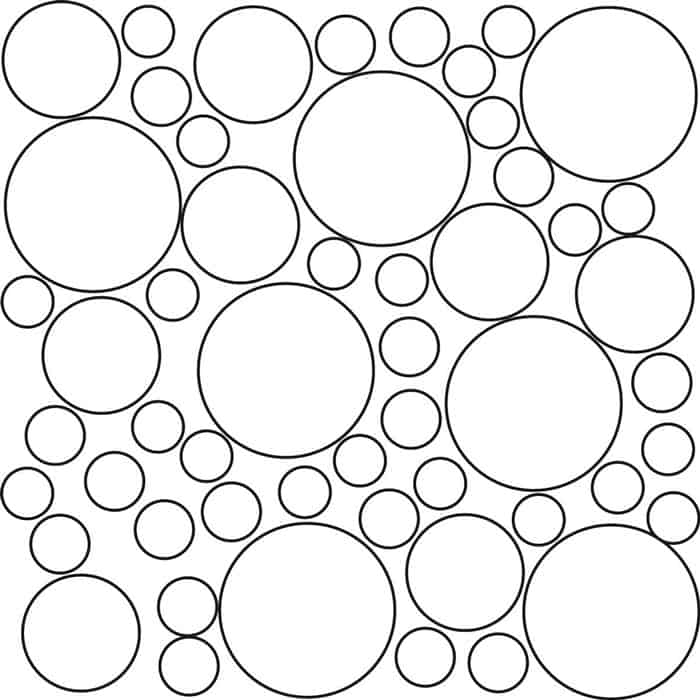
\includegraphics[width=2.5in]{figures/input-circles}\label{fig:input-circles}
  }
  \hfil
  \subfloat[Circles detected within the image.]{
  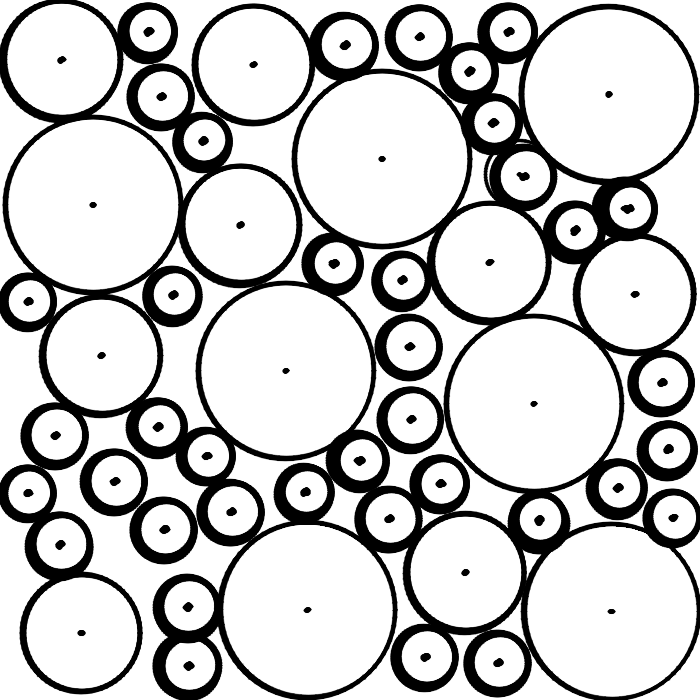
\includegraphics[width=2.5in]{figures/detected-circles}\label{fig:detected-circles}
  }
  \caption{\ref{fig:input-circles} is the input image that was used as an input to the program.\ref{fig:detected-circles} is the output to the program when it is run.}
\end{figure}

\section{\MakeUppercase{Methodology}}
\label{sec:Methodology}
\noindent
The HT implementation for our project detects circles that are present in an image compared to traditional line detection.
The HT itself is the population of a parameter space array, also referred to as an R-Table.
However, in order to run the population of the R-Table, multiple pre-processing routines are necessary to prepare the image for accurate shape detection.
The steps of the algorithm including pre-processing are color to grayscale conversion, edge detection, followed by population of the R-Table.
Our proposed method to implementing the HT includes using streaming in order to pipeline memory transfer with convolution calculations and R-Table population.

\begin{figure}
  \begin{itemize}
    \item RGB to Grayscale conversion of the input image.
    \item Image Blurring 
    \item Edge Map Generation
    \item Populate R-Table
  \end{itemize}\caption{Steps to conducting a Hough Transform on an image assuming an RGB image input.}\label{figure:hough-transform-steps}
\end{figure}

\subsection{RGB to Grayscale Conversion}
\noindent
Grayscale conversion of an image lends itself well to parallelization depending on the encoding of the image.
In our case, the input image used an RGB-RGB pixel ordering scheme, allowing for coalesced memory accesses from the GPU's global memory.

\subsection{Convolution}
\noindent
After generating the gray scale color space image, the majority of the algorithms used in image pre-processing for the HT can be applied via a convolution operation on the image.
Convolution is an algorithm that generates the convolution pixel by summing the element-wise multiplication of a source matrix and mask matrix as shown in \ref{equation:convolution}.

\begin{equation}
  m[x,y] * s[x,y] = \sum\limits_{i = 1}^{u} \sum\limits_{j = 1}^{v} m[i,j]s[x-i, y-j]
  \label{equation:convolution}
\end{equation}
Where $m$ is the mask matrix and $s$ is the source image matrix, $u$ and $v$ are the mask matrix dimensions. In our case, the mask matrices are square matrices.
Convolution is an algorithm that is readily parallelizable when implemented on a GPU, and as such, there were multiple optimizations that were made to extract as much performance as possible for image pre-processing.
Our convolution kernels were implemented in three iterations. 
A convolution kernel using global memory, one using constant memory for the mask, and a kernel utilizing shared memory stored in a 2D array.

\subsubsection*{Convolution Optimizations}
\noindent
Convolution is a high-priority algorithm for the researchers' implementation.
Blurring, edge detection, and thresholding all feature convolution as the main algorithm component.
After careful analysis, it was determined that there was potential  for parallelization.
This is because convolution features many independent multiplications, and GPUs are purpose built for these kinds of applications.

In first iteration of the convolution kernel, the goal is to translate the serial code into a parallel framework.
To do this, a naive approach shall be taken as a baseline.
Each thread is mapped to a single pixel image, meaning that for a m x n image, m x n threads are used.
Each thread accesses surrounding pixels, as well as the convolution kernel (or mask).
Finally, once the computation is done, the result is stored back in global memory by the thread.
Bounds checking is primordial to properly operate on images with dimensions not evenly divisible by the block size.

As will be discussed in a later section, this provided significant performance benefits.
However, further optimizations are possible.

As was covered in the GPU memory hierarchy overview in a previous section, we seek to exploit the benefits of GPU architecture to the fullest.
A big component of convolution is the continuous access of the convolution kernel.
As such, the next proposition was to transfer constant convolution kernels to the constant memory.
Transferring the entire image was not a possibility, as the constant memory is very limited in capacity.

While constant memory did provide a performance improvement it was relatively minor, and much lower than anticipated (as discussed further below).
To further improve performance,  a shared memory implementation was needed.
There were some challenges to this, as thread blocks require more memory elements than there are threads in the block.
To counter this, more thread blocks were launched with each block working on less amount of data.
This improved performance to acceptable levels.

By using a variety of masks across the images, it is possible to extract features or generate new kinds of maps that can be utilized by the HT\@.
Image denoising and gradient maps are both results of convolution operations with different masks.

\subsubsection*{Image Blurring}
\noindent
After the image is converted into grayscale color space, the image is de-noised by means of Gaussian blurring.
This aids in edge map generation by filtering our high frequency elements from the image.
To generate a blurred image, a convolution operation must be performed with a blurring mask. 
Our implementation uses a $5 \times 5$ Gaussian blurring mask where $\sigma = 1.4$ as shown in figure \ref{equation:gaussian5by5}.

\begin{figure} % puts the figure 'here'
  \centering
  $\begin{bmatrix}
  0.01 & 0.22 & 0.03 & 0.22 & 0.01 \\
  0.22 & 0.04 & 0.06 & 0.04 & 0.22 \\
  0.03 & 0.06 & 0.08 & 0.06 & 0.03 \\
  0.22 & 0.04 & 0.06 & 0.04 & 0.22 \\
  0.01 & 0.22 & 0.03 & 0.22 & 0.01 \\
\end{bmatrix}$\caption{A $5 \times 5$ Gaussian blurring mask where $\sigma = 1.4$}\label{equation:gaussian5by5}
\end{figure}

\subsubsection*{Gradient Map Generation}
After the image has been denoised by blurring, an edge map must be generated using two convolution operations using the horizontal (figure \ref{sub@equation:horizontalSobel}) and  vertical\ref{sub@equation:verticalSobel} variations of the Sobel operator as shown in figure \ref{figure:sobelOperator}.
\begin{figure} % puts the figure 'here'
  \centering
  \subfloat[Horizontal Operator]{
  $\begin{bmatrix}
    -1 && -2 && -1 \\
    0 && 0 && 0 \\
    1 && 2 && 1 \\
  \end{bmatrix}$\label{equation:horizontalSobel}
  }
  \hfil
  \subfloat[Vertical Operator]{
  $\begin{bmatrix}
    -1 && 0 && 1 \\
    -2 && 0 && 2 \\
    -1 && 0 && 1 \\
  \end{bmatrix}$\label{equation:verticalSobel}
  }
  \caption{A $3 \times 3$ Sobel Operator}\label{figure:sobelOperator}
\end{figure}

\subsubsection*{Grayscale Thesholding}
\noindent
After the convolution operation is performed with both masks the horizontal gradient $G_x$ and vertical gradient $G_y$ are generated. 
The gradient magnitude can be calculated using the gradient magnitude, $G$, as shown in figure \ref{equation:gradientMagnitude}.

\begin{equation}
  G = \sqrt{{G_x}^2 + {G_y}^2}\label{equation:gradientMagnitude}
\end{equation}

Image thresholding must be applied in order to generate the final edge map.
In our case, the thresholding value in our application was hard hard coded into our application where the value was chosen based off of experimentation for our application, as well as the problem domain for AZA.

\subsection*{Histogram Generation}
\subsubsection*{R-Table Generation}
Image pre-processing has been completed after the edge map has been generated and binarized via graycale threshold segmentation.
The next part of the algorithm is population of the R-Table in order to parameterize the circles that are present in the image.
\subsubsection*{Populate R-Table}
The parameter space, also referred to as an R-Table, contains 3 bins to parameterize a circle.
\begin{equation}
  X_{i}, Y_{i}, R_{i}\label{circle-parameters}
\end{equation}
Where $X_i$ and $Y_i$ are the center coordinates and $R_i$ is the radius of the detected circle.
In a serial implementation, one would cycle through each possible parameter and check how many edge pixels are present along the parameterized shape. 
A count of matching pixels is then accumulated for each bin in the parameter space.
After the R-Table is populated with the corresponding parameters, the HT algorithm itself has terminated to completion.
The generation of the R-Table has a histogram like implementation where many data are being transported to one location.

\subsection*{Histogram Generation Optimizations}
The R-Table parameterization was implemented in three ways. A global memory implementation, a local accumulator implementation, and a shared memory implementation.
The first implementation generates the R-Table by mapping each thread to a separate radius.
Generation of the histogram in a paralleled fashion has trade-offs that must be addressed. 
In the initial implementation, each thread is responsible for a populating the parameters in a separate bin, that is, the data was transformed in a gathering pattern. 
The second iteration of the R-Table population operation implemented a local accumulator variable in place of an atomic add operation, only running an atomic add after completion of the parameterization.
In theory, this reduces the amount of memory contention that is present within the R-Table stored on the GPU\@.
However, since each thread populates a different parameter, the data access pattern has low memory contention.
Thus, mostly nullifying the benefits of a local accumulator that would be present if the algorithm implementation contained greater memory contention.
After examining the data access pattern, it can be concluded that the bottleneck in the algorithm is the with the manipulation of the histogram, but instead lies in the speed at which image data is accessed.
This led to the next proposed optimization to be including the use of shared memory within a thread block.
The third implementation uses each thread to copy the image onto shared memory, decreasing the amount of time that would be required to access the image.
However, the shared memory was not sufficient to contain the entire image when using the current algorithm.

\subsubsection*{Addressing Shared Memory Storage Limits}
There are two methods proposed to address this storage space issue. 
The first way to address the issue is by down sampling the image to reduce the image size, making sure to de-noise the image in the down-sampling process. 
By down sampling the image, the image may be capable of fitting on the GPU's shared memory dependent on the application.
Our GPU, has a shared memory size of 64kB.
Down-sampling by a factor of 4, reduces the $700 \times 700$ 8-bit image to a total of 122.5kB of data. 
This reduction in image size however, is still not sufficient. 

\subsubsection*{Changes to The Histogram Generation Algorithm}
In order to allow the image to fit on shared memory, the thread workload must be modified.
By splitting the circles into four quadrants, each thread block loads only a quarter of the image, reducing the amount of memory space required for each memory block to 30.625kB. 
This algorithm while allowing for faster memory accesses than global memory after the image has been loaded on to hardware is quite directly translated from a serial implementation.

\subsubsection*{A Different Kind of Implementation}
The previous implementations of the algorithm thread number as the center of the circle and scan all image pixels that should be a part of the circle.
While this implementation is very direct, it is is heavily bottle-necked by memory accesses. 
To reduce memory accesses conducted by all threads, the algorithm used to populated the histogram can be heavily modified.
Instead of using thread location to determine the center of the circle, each thread can check the image for an edge pixel. 
If the thread detects that an edge pixel is present, the histogram bin pertaining to all possible circles that house that edge pixel can be incremented.
This optimization allows a local accumulator to have a greater effect on the execution time because memory contention would increase among the thread blocks and histogram. 
This algorithm would also make traditional histogram population optimization such as private histograms produce greater speedups.
This change in the algorithm increases computation time in proportion to memory transfer time, better utilizing GPU resources as well as optimizing the kernel for the use of CUDA streaming.
Due to time constraints and lack of manpower, this algorithm was not implemented in this project.

\subsection*{Cuda Streaming}
With the individual algorithms optimized, this project was nearing completion. However, upon speaking to other teams and our PI, it was evident that system resources were not being utilized to the fullest. Even for pre-processing alone, the ratio of computation time to memory transfer time was approximately 1.4:1.0. This presents an interesting scenario, as it means that the memory unit remains idle while computations happen. As such, a potential opportunity for streaming had been found.
Creating a streaming implementation is simultaneously an easy task and a complicated one. It is easy to implement because it does not require any changes to individual kernels. However, plenty of the main code needed changes, such as changing mallocs to cudaHostAlloc(), creating for loops for streams, among a plethora of changes.
To perform this analysis, two experiments were done. The first one involves running all the pre-processing on several streams, while the second experiment was streaming on the entire algorithm. Results are reflected below, however they were not as good as hoped.

\section{\MakeUppercase{Evaluation and Validation}}
\begin{figure}
\begin{center}
\begin{tabular}{ |c|c|c|c|} 
 \hline
 Serial & Naive & Constant Mem & Shared Mem \\ 
 \hline
 129.76 ms & 0.1546 ms & 0.1416 ms & 0.09843 ms\\
 \hline
\end{tabular}\caption{Table of speedup results from individual convolution optimizations}\label{table:convolutionTimes}
\end{center}
\end{figure}
\subsection{Convolution Optimizations}

As seen from the previous table (figure \ref{table:convolutionTimes}), GPU optimization of convolution was a success! The convolution speedup test involved running convolution on a 720x1280 image witha 5x5 kernel on each of the described methods 10 times, and taking the average of all the attempts for each category. Note that the shared memory implementation is not a standalone implementation. Rather, it is built upon the constant memory implementation as well. 
\begin{figure}
\centering
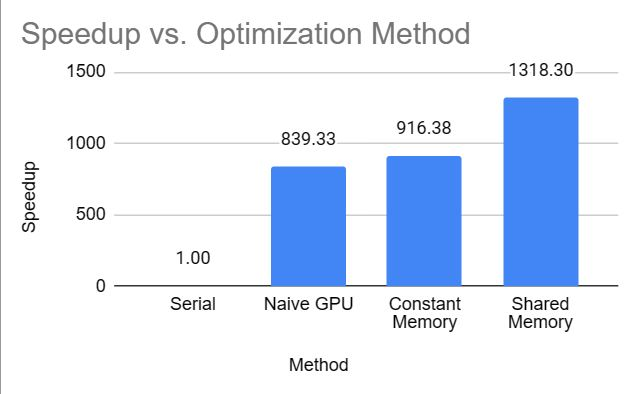
\includegraphics[width=2.5in]{figures/ConvolutionSpeedup}\caption{Speedup amount vs serial implementation.}\label{figure:convolution-speedup}
\end{figure}
Of noteworthiness is the fact that constant memory did not produce the anticipated results. On the naive implementation, each pixel requires 25 global memory reads for the kernel. Multiply that by the total amount of pixels, and a big reduction in global memory reads is achieved. However, performance improvement when compared to a naive GPU implementation was only a 1.09x speedup. The possible reason is that, due to the frequent accesses to memory, data has already been cached. Therefore, constant memory only presented a marginal improvement. 
On the other hand, a shared memory implementation provides a successful improvement, being approximately 1.44x faster than constant memory version. Further performance increase may be obtained by reducing thread divergence, but that was beyond the scope of this project.

\subsection{Histogram Population Optimizations}
As previously stated, the algorithms that were implemented on the GPU include the naive approach, which accesses global memory to retrieve edge pixel information.
The second implementation removes atomic add operations from the inner loops and uses a local accumulator.
The third implementation attempts to load the image into shared memory. However, because of shared memory size constraints, the third implementation was unsuccessful.

\begin{figure}
\begin{center}
\begin{tabular}{ |c|c|c| } 
 \hline
 Serial Implementation & Naive GPU & Local Accumulator \\ 
 \hline
 284362 s & 4.090 s & 4.067 s \\
 \hline
\end{tabular}\caption{Table of speedup results from R-Table Implementations}\label{table:histogramGeneration}
\end{center}
\end{figure}

As seen in figure \ref{table:histogramGeneration}, the serial implementation, run on an Intel Core i7 8700k @ 3.7 GHz executed the population of the R-Table in approximately 284.36 seconds.
The first implementation, utilizing the global memory on the GPU using global memory and an atomic add operation within the loop executed the population of the R-Table in approximately 4.090 seconds.
This second implementation on the GPU executed the population of the R-Table in approximately 4.067 seconds.
Speedup from the serial implementation to the naive GPU implementation is 69.5x.
Speedup from the naive GPU implementation to the local accumulator memory is negligible. 
The reason for this being the case has to do with the fact that each thread is tied to one set of parameters at any given time.
Different parameters are being populated by different threads there is no memory contention among atomic operations. 
Changing the algorithm to require less image accesses per thread and instead focusing on populating individual parameters would have been a more fruitful approach to optimizing this step of the HT algorithm.\label{section:histogramGeneration}

\subsection{Streaming}
As mentioned beforehand, streaming was a consideration for a possible performance improvement. While streaming does not increase latency for a single image, it increases overall throughput by pipelining the kernels. The first experiment involves a streaming implementation of all pre-processing kernels, namely Grayscaling, and three convolution kernels, on a set of 60 images. Timing and performance analysis was done, and the throughput measurement includes memory transfer overhead (sending image for kernel operations, and retrieving the output). Here are the results:
\begin{figure}
\centering
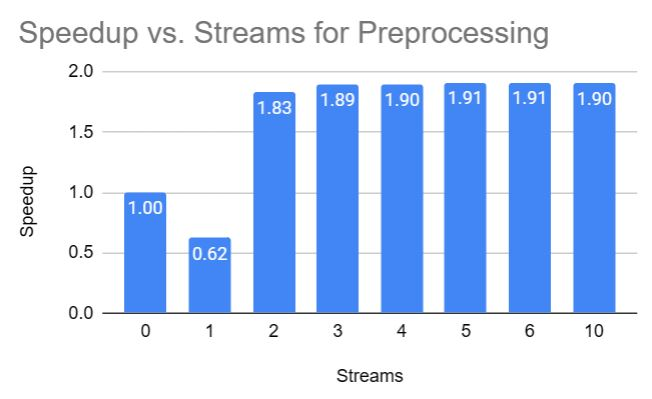
\includegraphics[width=2.5in]{figures/StreamingPreProcessing}\caption{Speedup vs \# of streams for pre-processing}\label{figure:streamPreProcess}
\end{figure}

Seeing the potential success of streaming, the decision was made to create a streaming implementation for the whole algorithm. The initial expectations were that performance improvements would exceed that of the pre-processing speedups. As such, a secondary experiment was realized with the entire process streamed, the entire algorithm with 30 images was executed 10 times for each stream amount.

\begin{figure}
\centering
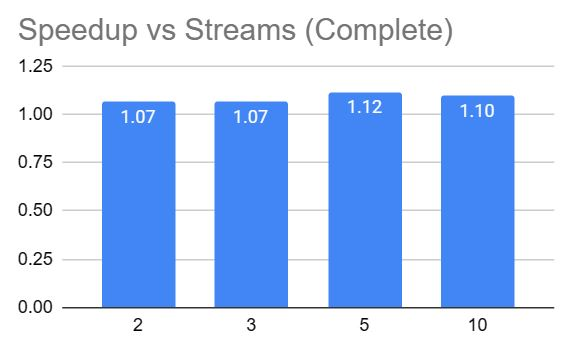
\includegraphics[width=2.5in]{figures/StreamsComplete}\caption{Speedup vs \# of streams for complete process}\label{figure:streamComplete}
\end{figure}

As shown in figure \ref{figure:streamComplete}, results were not as anticipated. Streaming provided less of a performance improvement than predicted, and by quite a large margin. Upon a root analysis cause, it was determined that the computation time on the Hough Transform far exceeded both pre-processing and memory transfer overhead. Therefore, any performance improvement was largely small in comparison to the Hough Transform. This means that the goal performance of 30 FPS was not met.

\section{\MakeUppercase{Conclusion}}

After careful analysis of research results, methodology used and target architecture, it is clear that potential for image processing acceleration through GPU-based systems is high. A significant increase in performance for shape detection (when compared to a serial implementation) was seen. Exploiting the software features allows for not only increased performance in parallel floating point operations, but also a familiar  development process for people with experience in common programming languages. As has been the case for years, GPU hardware features prove particularly well-suited for image processing applications due to their parallel nature. GPU interest and development has skyrocketed in recent years, allowing for even further research as well as new hardware features and simplified software development.

However, research findings are not completely positive as top performance targets were not met. While theoretical and predicted results were within the desired range, a combination of unexpected hardware limitations (including but not limited to shared memory and number of available SMs), highly optimistic goals, and external circumstances, all led to results that did not reach the ideal values. Streaming implementation did not have the anticipated bandwidth and performance results.

Reccomendations for future work in the field of GPU-accelerated image processing include rethinking the approach of several common techniques, such as Hough transform, to better align with the hardware limitations and target architecture. Furthermore, batching is reccomended as the next algorithmic improvement to research on.

\subsection{Acknowledgements}

We would like to thank Dr. Marcellin, Dr. Akoglu and The University of Arizona for their support and invaluable resources when completing this research paper.

\bibliographystyle{ieeetr}
\bibliography{references.bib}
\end{document}
